\iffalse
\documentclass[12pt]{article}
\usepackage{graphicx}
%\documentclass[journal,12pt,twocolumn]{IEEEtran}
\usepackage[none]{hyphenat}
\usepackage{graphicx}
\usepackage{listings}
\usepackage[english]{babel}
\usepackage{graphicx}
\usepackage{caption}
\usepackage[parfill]{parskip}
\usepackage{hyperref}
\usepackage{booktabs}
%\usepackage{setspace}\doublespacing\pagestyle{plain}
\def\inputGnumericTable{}
\usepackage{color}                                            %%
    \usepackage{array}                                            %%
    \usepackage{longtable}                                        %%
    \usepackage{calc}                                             %%
    \usepackage{multirow}                                         %%
    \usepackage{hhline}                                           %%
    \usepackage{ifthen}
\usepackage{array}
\usepackage{amsmath}   % for having text in math mode
\usepackage{parallel,enumitem}
\usepackage{listings}
\lstset{
language=tex,
frame=single,
breaklines=true
}
%Following 2 lines were added to remove the blank page at the beginning
\usepackage{atbegshi}% http://ctan.org/pkg/atbegshi
\AtBeginDocument{\AtBeginShipoutNext{\AtBeginShipoutDiscard}}
%
%New macro definitions
\newcommand{\mydet}[1]{\ensuremath{\begin{vmatrix}#1\end{vmatrix}}}
\providecommand{\brak}[1]{\ensuremath{\left(#1\right)}}
\providecommand{\abs}[1]{\left\vert#1\right\vert}
\providecommand{\norm}[1]{\left\lVert#1\right\rVert}
\newcommand{\solution}{\noindent \textbf{Solution: }}
\newcommand{\myvec}[1]{\ensuremath{\begin{pmatrix}#1\end{pmatrix}}}
\let\vec\mathbf
\begin{document}
\begin{center}
\title{\textbf{ Intercepts Lines}}
\date{\vspace{-5ex}} %Not to print date automatically
\maketitle
\end{center}
\setcounter{page}{eq:11/10/4/31}
\section*{11$^{th}$ Maths - Chapter 10}
This is Problem-3 from Exercise 10.4
\section{Solution}
\fi
Let the $x$ intercept be $a$ and  the $y$ intercept be $b$ ,Then
\begin{align}
a+b&=1\label{eq:11/10/4/31a}\\
ab&=-6 \label{eq:11/10/4/32a}
\\
\implies  a = 3, b = -2
\end{align}
Thus, the possible 
intercepts are
\begin{align}
\myvec{3\\0}, \myvec{0\\-2},
\myvec{-2\\0}, \myvec{0\\3}
\end{align}
yielding
\begin{align}		
\vec{m}=\myvec{3\\2} \text{or,} \myvec{-2\\3}
\end{align}
\begin{enumerate}
\item For 
\begin{align}
\vec{n}
=\myvec{-2 \\3} 
\end{align}
the equation of the line is 
\begin{align}
	\vec{n}^\top\brak{\vec{x}-\vec{A}} &= 0 \\
	\myvec { -2 & 3 } \vec{x}  &= 6  
\end{align}
\item  For 
\begin{align}
\vec{n}
=\myvec{-3 \\-2} 
\end{align}
the equation of the line is 
\begin{align}
    \vec{n}^\top\brak{\vec{x}-\vec{B}} &= 0 \\  
	\myvec { -3 & -2 }  \vec{x}  &= 6        
\end{align}
\end{enumerate}
See Fig. 
\ref{fig:11/10/4/3line segmenta}.
\begin{figure}[h!]
\centering
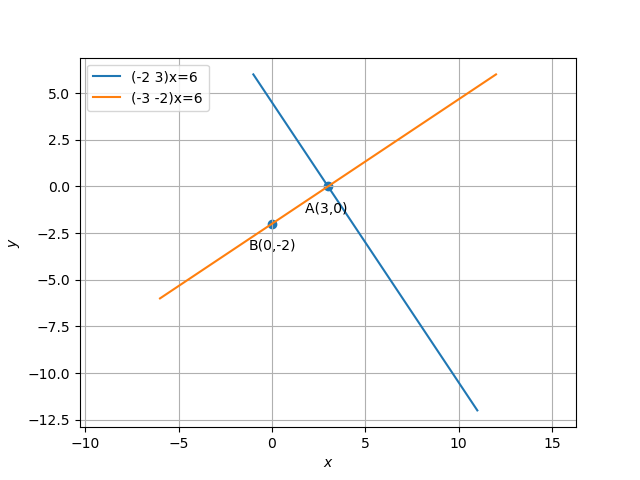
\includegraphics[width=\columnwidth]{chapters/11/10/4/3/figs/inter.png}
\caption{}
\label{fig:11/10/4/3line segmenta}
\end{figure}
